% easychair.tex,v 3.2 2012/05/15
%
% Select appropriate paper format in your document class as
% instructed by your conference organizers. Only withtimes
% and notimes can be used in proceedings created by EasyChair
%
% The available formats are 'letterpaper' and 'a4paper' with
% the former being the default if omitted as in the example
% below.
%
\documentclass{llncs}
%\documentclass[debug]{easychair}
%\documentclass[verbose]{easychair}
%\documentclass[notimes]{easychair}
%\documentclass[withtimes]{easychair}
%\documentclass[a4paper]{easychair}
%\documentclass[letterpaper]{easychair}

% This provides the \BibTeX macro
\usepackage{doc}
\usepackage{makeidx}
\usepackage{fancyvrb}
\usepackage{listings}
\usepackage{longtable}
\usepackage{paralist}
\usepackage{color}
\usepackage{algpseudocode}
\usepackage{hyperref}
\usepackage{graphicx}
\usepackage{amsmath}
\hypersetup{
    colorlinks,
    citecolor=black,
    filecolor=blue,
    linkcolor=black,
    urlcolor=blue
}

% Let's style the code!
% Set-up code visualisation
\lstset{fancyvrb=true}
\lstset{
language=java,                % the language of the code
basicstyle=\footnotesize,       % the size of the fonts that are used for the code
numbers=left,                   % where to put the line-numbers
numberstyle=\footnotesize,      % the size of the fonts that are used for the line-numbers
stepnumber=1,                   % the step between two line-numbers. If it's 1, each line 
                                % will be numbered
numbersep=5pt,                  % how far the line-numbers are from the code
keywordstyle=\color{blue},
commentstyle=\color{green},
stringstyle=\color{red},
backgroundcolor=\color{white},  % choose the background color. You must add \usepackage{color}
showspaces=false,               % show spaces adding particular underscores
showstringspaces=false,         % underline spaces within strings
showtabs=false,                 % show tabs within strings adding particular underscores
frame=single,                   % adds a frame around the code
tabsize=2,                      % sets default tabsize to 2 spaces
captionpos=t,                   % sets the caption-position to bottom
breaklines=true,                % sets automatic line breaking
breakatwhitespace=false,        % sets if automatic breaks should only happen at whitespace
%title=\lstname,                 % show the filename of files included with \lstinputlisting;
                                % also try caption instead of title
escapeinside={\%*}{*)},         % if you want to add a comment within your code
morekeywords={*,...}            % if you want to add more keywords to the set
}
\lstset {
    keywordstyle=\color[rgb]{0,0,1},          % keywords in blue
    commentstyle=\mcommentfont,               % comments
    stringstyle=\color[rgb]{.627,.126,.941},  % strings in purple
    commentstyle=\color[rgb]{.133,.545,.133}
}

% In order to save space or manage large tables or figures in a
% landcape-like text, you can use the rotating and pdflscape
% packages. Uncomment the desired from the below.
%
% \usepackage{rotating}
% \usepackage{pdflscape}

% If you plan on including some algorithm specification, we recommend
% the below package. Read more details on the custom options of the
% package documentation.
%
% \usepackage{algorithm2e}

%\makeindex

%% Document
%%
\begin{document}

%% Front Matter
%%
% Regular title as in the article class.
%
\title{Ensuring Faultless Communication Behaviour\\
       in an E-Commerce Cloud Application}

% \titlerunning{} has to be set to either the main title or its shorter
% version for the running heads. When processed by
% EasyChair, this command is mandatory: a document without \titlerunning
% will be rejected by EasyChair

\titlerunning{Faultless Commuication in a Cloud}

% Authors are joined by \and. Their affiliations are given by \inst, which indexes
% into the list defined using \institute
%
\author{
	Rustem A. Kamun \and Ross Horne
}

% Institutes for affiliations are also joined by \and,
\institute{
  Kazakh-British Technical University, 
  Faculty of Information Technology,\\
  Almaty, Kazakhstan\\
  \email{r.kamun@gmail.com}
 }
%  \authorrunning{} has to be set for the shorter version of the authors' names;
% otherwise a warning will be rendered in the running heads. When processed by
% EasyChair, this command is mandatory: a document without \authorrunning
% will be rejected by EasyChair

\authorrunning{Kamun \& Horne}


%\clearpage

%%%%%%%%%%%%%%%%%%%%%%%%%%%%%%%%%%%%%%%%%%%%%%%%%%%
\maketitle
%%%%%%%%%%%%%%%%%%%%%%%%%%%%%%%%%%%%%%%%%%%%%%%%%%%

\begin{abstract}
  An increasing scope and complexity of Web services raises a new challenge of controlling their interaction. The goal of this work is to ensure that processes in a production Cloud are correctly interacting according to a specification of their communication behaviour. To accomplish this goal, we employ session types to analyse the global and local communication patterns. Session types represents ``formal blueprints" of how communicating participants should behave and offers a concise view of the message flows.
  
  This work confirms the feasibility of application of session types on ``non-linear'' business protocols used by an e-commerce Cloud provider and developed in Session-Java, an extension of Java implementing Session-Based programming. Furthermore, we highlight the importance of this approach for services replicated across multiple Cloud providers each of which must correctly cooperate.
\end{abstract}

%\setcounter{tocdepth}{2}
%{\small\tableofcontents}

%\section{To mention}
%
%Processing in EasyChair - number of pages.
%
%Examples of how EasyChair processes papers. Caveats (replacement of EC
%class, errors).

%\pagestyle{empty}


%------------------------------------------------------------------------------
\section{Introduction}
\label{sect:introduction}

%The growing needs for information availability and accessibility present new challenges for application development.
The need for highly available services presents challenges for application development.
There are two forces working in parallel with regards to the need for integration.
First, the necessity of application integration within a company (enterprise), and second, business-to-business integration.
There is an increasingly widespread acceptance of Service-Oriented Architectures (SOA) as a paradigm for integrating software applications within and across organizational boundaries.
In this paradigm, independently deployed applications are exposed as (Web) services which are then 
interconnected using a stack of standards, which depicted in Figure~\ref{fig:soa-stack}. 
		
		\begin{figure}[ht]
		\begin{centering}
		\scalebox{0.7}{
		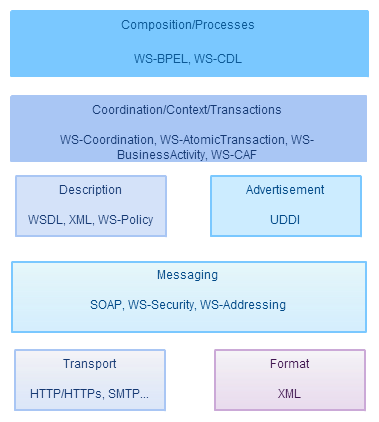
\includegraphics[width=0.5\textwidth]{WS_stack.png}
                }
		\caption{Stack of WS Standards}
		\label{fig:soa-stack}
		\end{centering}
		\end{figure}
		
However there remain open challenges when it comes to managing service interactions that go beyond simple sequences of requests and responses or involve large numbers of participants (multi-party communication). A need arises for new transaction implementations, more suitable for the web. One of those techniques for describing collaboration between a collection of services is a choreography model. It captures the interactions in which the participating services engage and interconnections between these interactions, including control-/data-flow dependencies. However, a choreography does not describe any internal action that occurs within a participating service. In turn, we do not have a clear idea how a global description can be executed, and, therefore, its functionality is not clear.

Much literature exist on the specification of systems that describe serives from the local viewpoint~\cite{cs-processes,alg-seq-processes}. In addition there is no special concept of the participants of communication. It is especially essential in complex interactions that take place today: 

	\begin{compactenum}
	   \item business transactions with short life span, operating in closely coupled context, where SOA standards may become a trap (online stock exchange(ForEX), services based on BSH protocol\footnote{Buyer-Seller-Shipper protocol} such as e-commerce services);
	   \item applications with a long life span that may result in deadlock.
	\end{compactenum}
These are the motivation under the design of WS-CDL (Web Services Choreography Description Language). However, WS-CDL working group discovers its issues that are critically exposed in \cite{ws-critical-overview}:
\begin{compactenum}
	\item tools to validate conformance to choreography specifications to ensure correct cooperation between web services;
	\item design time validation and verification of choreographies to guarantee correctness of such properties like deadlock, livelock e.g. behaviour of participants conforms to the choreography interface.
\end{compactenum}
Aforementioned challenges can be tackled under a strong theoretical foundations. Fortunately, successful attempts has already made by F. Montesi, M. Carbone who developed Chor programming language \cite{chor-lang,carbone2013deadlock} based on sessions and theory of trace sets~\cite{chor-essence}, and N. Yoshida, K. Honda developed Session-Java language \cite{sj-lang}, based on session types \cite{session-types-sessions,carbone2007structured}.

In this paper we will demonstrate a method of controlling process interactions represented by sessions. The formal theory based on session types ensures communication safety by verifying that session implementations of each engaged participant conform to the defined protocol specification. In order to prove the feasibility of this theory we utilized Session-Java, an extension to Java language. It works by specifying the intended process transaction protocol using session types and implementing the interaction using session operations.

In Section~\ref{sect:basics} we provide fundamentals of SJ syntax and features.
Next, in Section~\ref{sect:impl}, we provide detailed explanation of business protocols used by an e-commerce Cloud provider\footnote{\url{http://v3na.com}. Cloud platform for optimizing your business performance.}. %~\cite{v3na-cloud}. Make this citation a footnote.
Finally, in Section~\ref{sect:highlights} we highlight an idea to use session types in designing Intercloud~\cite{intercloud} communication protocols.

Through these we are aiming to confirm the suitability of Session-Java as an implementation of business to business transactions. We want to explore the agility and robustness of the language and the scalability as scenarios vary in size but also complexity. In addition we will be looking for things such as ease of programming in SJ, any limitations, bugs or non-implementable scenarios.

%------------------------------------------------------------------------------
\section{Basics of Session-Java}
\label{sect:basics}

Session programming begins from the protocols specification for interaction (using session types), which can then be concretely implemented using a set of structured communication operations available on session sockets. Session programming is applicable for applications where the parties or components cooperate according to specified protocols: session types are formal specifications of such protocols. Session types describe structured sequences of interaction including basic message passing, branching, branching and repetition. A session is an instance of a session type, i.e. the unit of interaction encapsulating one run of a protocol. From the perspective of abstraction, each session, is conducted on a separate channel. 

Session programming in SJ consists of the following ordered actions:

\begin{compactenum}
  \item design specification (protocol) of target communication;
  \item mapping protocols into the programs for each participant. For instance, in BSH protocol, we can distinguish three main participants whose actions (processes) are mapped to corresponding programs (software component);
  \item By utilizing session programming constructs, implementing the protocol, where each operation is performed as method call;
  \item verification of sessions fulfilment by  compiler;
  \item execution and system testing.
\end{compactenum}

\subsection{Protocol Specification}
Session programming begins by declaring the protocol for the intended cooperation as follows:

\begin{equation*}
\text{protocol name \{\dots\}}
\end{equation*}
where name identifies the protocol, following the standard Java naming rules. The body of the protocol is \textit{session type}, given by the syntax rules in Table \ref{tab:prot-spec}, below.

\begin{longtable}{|p{0.15\textwidth}|p{0.3\textwidth}|p{0.3\textwidth}|}
\caption{SJ protocol specification}\label{tab:prot-spec} \\
\hline
$T$ & $::=T.T$ & Sequencing \\ \hline
& begin & Session initiation \\ \hline
& $!<M>$ & Message send \\ \hline 
& $?(M)$ & Message receive \\ \hline
& $\oplus \{L_1:T_1,\dots, L_n:T_n \}$ & Session branching \\ \hline
& $\oplus [T]*$ & Session iteration. \\ \hline 
& $\text{rec }L[T]$ & Session recursion scope. \\ \hline
& \#$L$ & Recursive jump. \\ \hline
& @$p$ & Protocol reference. \\ \hline
\end{longtable}

The session type shows how a session should be designed in terms of actions that the participant should perform. The key point is that the implementation of a session is governed by associated protocol: the SJ compiler (Polyglot\footnote{Extensible compile framework available at \url{http://www.cs.cornell.edu/Projects/polyglot/}}). It can be clearly seen from the Table \ref{tab:prot-spec}, that SJ has enough constructs to describe diverse range of complex interactions: message passing, conditional and repeated expressions. Its worth noting, that each session type element has its dual element, because there is a requirement that two parties implement compatible protocol such as the specification of one party has dual relation to another party.

\subsection{Higher Order Communication}
In order to describe richer behaviour, SJ has a feature of subtyping. It means that message types can themselves be session types. It also enhances the agility of the type system by allowing the participants in a session to follow different protocols which are compatible \cite{higher-order-comm}. Such communication can be expressed by the following dual constructs:

\begin{equation*}
!<?(\text{int})> \hspace{2cm} ?(?(\text{int}))
\end{equation*}

In short, it says that we are expected to send and receive a session of type ?(int). Higher order communication, as we will convince further, is often referred to a session delegation. Figure \ref{fig:sj-delegation} shows a basic delegation scenario.

\begin{figure}[ht]
\centering
\scalebox{0.7}{
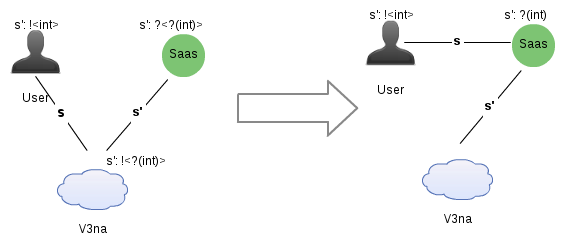
\includegraphics[width=0.8\textwidth]{sj-delegation.png}}
\caption{Session delegation}\label{fig:sj-delegation}
\end{figure}

The left part illustrates the session configuration before the delegation is performed: User engaged in a session $s$ of type $!<$int$>$ with V3na (Cloud), while Cloud is also involved in a session $s'$ with SaaS of type $!<?($int$)>$. So, instead of accepting the integer from User himself, Cloud delegates his role in $s$ to SaaS, so that he will receive this message. This delegation action corresponds to higher-order send type for the session $s'$ between Cloud and SaaS. The right part of figure illustrates the change in session configuration after the delegation has been performed: User now directly interacting with SaaS for the session $s$.

\subsection{Protocol Implementation using Session}
\paragraph{Another meaning for sockets}
Session sockets are implementing the actual session code according to the specified session type (protocol). They are represent the endpoints (participants) of a session connection: each of the parties owns one endpoint and performs the specified interactions via the SJ session operations on that endpoint. In SJ session sockets are objects that extend the abstract \textit{SJSocket} class. \textit{SJRSocket::SJSocket} and \textit{SJFSocket::SJSocket}, both, employ TCP as underlying transport. SJ is distinguishing session client and server sockets, where the former are used to request sessions from the latter.

\paragraph{Session operations}
After creating a protocol (session type) and encapsulating the session into SJ socket, it can be implemented within a session-try scope using the session operations depicted in Table \ref{tab:session-ops}.

\begin{longtable}{|p{0.4\textwidth}|p{0.4\textwidth}|}
\caption{Session operations specification}\label{tab:session-ops}\\ \hline
s.request() & begin \\ \hline 
s.send(m) & $!<M>$ \\ \hline
s.receive() & $?(M)$ \\ \hline
s.outbranch(L) \{P\} & $!\{L:T\}$ \\ \hline
s.inbranch() \{case L1: {P1}\dots case Ln:{Pn}\} & $?\{L_1:T_1,\dots, L_n:T_n\}$ \\ \hline
s.outwhile(cond) \{P\} & $[T]*$ \\ \hline
s.inwhile() \{P\} & $?[T]*$ \\ \hline
s.recursion(L) \{P\} & rec $L[T]$ \\ \hline
s.recurse(L) & $\#L$ \\ \hline
\end{longtable}

The session operations are invoked via session in a method call-like manner. To delegate a session, the session socket variable must be passed to a send operation on the target session.

\begin{lstlisting}
s1.send(s2) // !<T>, where T is the remaining session type of 's2'
\end{lstlisting}


Only active session sockets can be delegated. The receive operation receives delegated sessions:

\begin{lstlisting}
SJSocket s2 = s1.receive()
\end{lstlisting}

%------------------------------------------------------------------------------
\section{Business case studies}
\label{sect:impl}

V3na.com is an e-commerce web portal that sells SaaS applications for business needs. V3na has developed on Django framework (Python)\footnote{ Django is a high-level python web framework that encourages rapid development and clean. Further information: \url{https://www.djangoproject.com/}}. The persistence layer is based on MongoDB and Memcached. One of the challenging task was to automate the process of SaaS integration. By integration we understand the following processes with a particular SaaS application:

\begin{compactitem}
\item  connection: SaaS user can connect SaaS for trial period by simply clicking on the button;

\item  subscription extension and freezing;

\item  payment confirmation;

\item one entry point to all user's applications.
\end{compactitem}
Full source  code is available at \url{https://github.com/Rustem/Master-thesis}.

\subsection{Simple Scenario}
\paragraph{Protocol declaration} As a starting point, let's specify simple business protocol of one of the processes just mentioned, SaaS connection. Informally, it may be interpreted as follows:
\begin{enumerate}
\item  User begins a request session (s) with cloud service (V3na) and sends the request ``Connect SaaS'' as JSON-encoded message.

\item  V3na sends either:

\item  FAIL, if user has no active session (not signed in on V3na) and further interaction terminates 

\item  OK, if user has logged in and request data has passed validation steps. Then Cloud initiates a new session (s') with SaaS and requests it for new user connection with HttpRequestJSONMessage.

\item  If OK label take place, Cloud initiates a new session (s') with SaaS and requests it for new user connection with HttpRequestJSONMessage. finally SaaS responds to Cloud with connection status (OK, FAIL) and V3na sends this status to User. Both sessions have to be terminated.
\end{enumerate}

\textit{Protocols.} The decision in the protocol will be incorporated through the use of outbranch. So the whole scenario is presented on Table \ref{tab:protocols-sc1}.

{
\lstset{
framerule=0pt,
numbers=none
}
\begin{longtable}{|p{0.3\textwidth}|p{0.3\textwidth}|p{0.3\textwidth}|}
\caption{Protocols of scenario \# 1}
\label{tab:protocols-sc1} \\ \hline
User & Cloud (V3na) & SaaS \\ \hline
\endhead

\begin{lstlisting}
protocol p_uv { 
  begin.
  !<JSONMessage>. 
  ?{
    OK: ?(JSONMessage).?(int),
    FAIL: 
  }
}
\end{lstlisting}
&
\begin{lstlisting}
p_vu { 
  begin.?(JSONMessage).!{
    OK: !<JSONMessage>.!<int>,
    FAIL: 
  }
protocol http_req_rep {
  !<JSONMessage>.
  ? (JSONMessage)
}
protocol p_vs { 
  begin.@http_req_rep 
}
\end{lstlisting}
&
\begin{lstlisting}
protocol p_sv { 
  begin.
  ?(JSONMessage). !<JSONMessage> 
}
\end{lstlisting}
\\ \hline
\end{longtable}
}

\paragraph{Interactions.} The general syntax for global description has been interpreted into a sequence UML diagram, as depicted in Figure \ref{fig:interaction-overview-sc1}. The whole syntax is on the down-left side of the figure. In case of choice, terminated branches are out of scope of the main picture, but still a subpart of the whole diagram. Next step is implementation of this diagram in Session-Java.

\begin{figure}[ht]
\centering
\scalebox{0.3}{
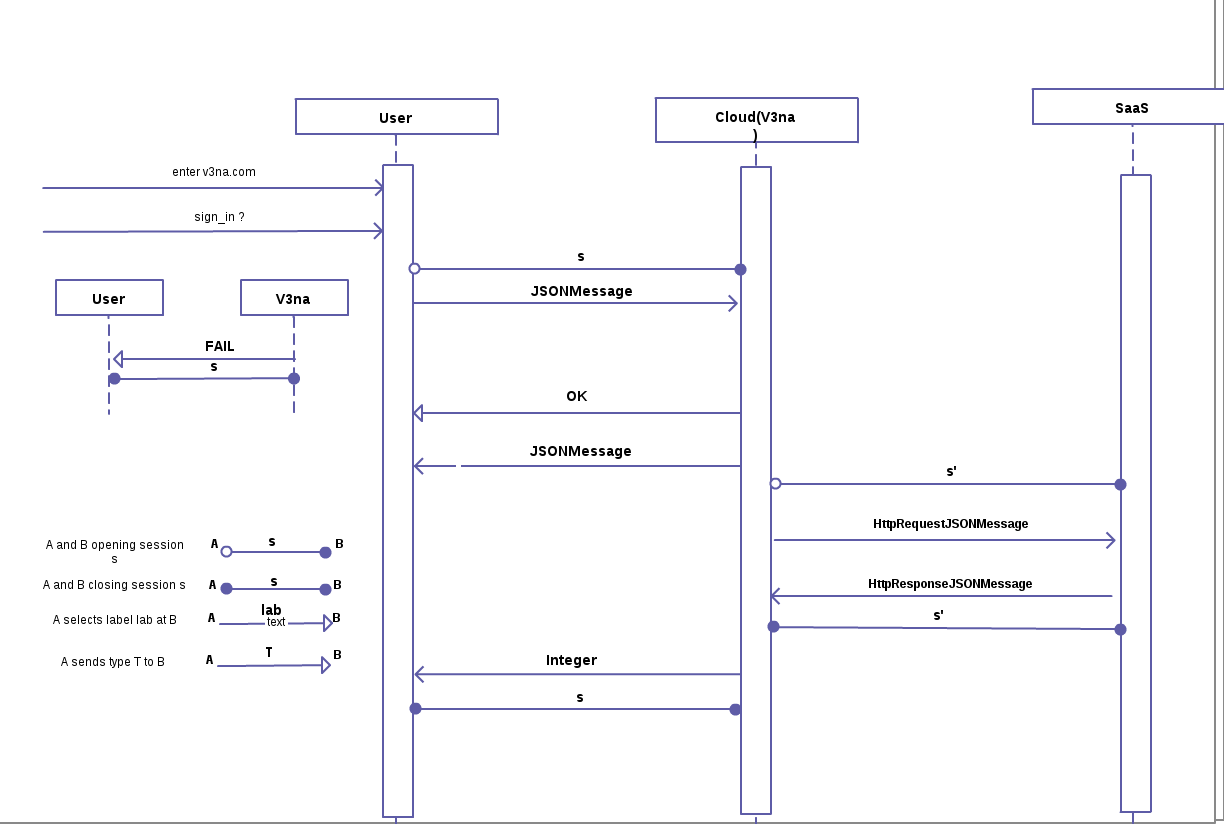
\includegraphics{interaction-sc1.png}}
\caption{Overview of interactions for Scenario \# 1}
\label{fig:interaction-overview-sc1}
\end{figure}

The main feature of SJ in this scenario is that choice can be expressed by using \textit{outbranch} construct.

\subsection{Complicated Scenario}
New scenario is a bit harder in complexity. We are going to utilize looping construct as well as demonstrating \textit{session delegation}. The description of the scenario of this subsection presented below as follows:
\begin{compactenum}
\item  User begins a request session (s) with cloud service (V3na)

\item  V3na asks User to login, so next User provides V3na with login and password Strings.

\item  V3na receives User credentials and verifies them: If User is authenticated with minimal amount of tries or amount of tries is out of limit, he is allowed to continue further interactions with V3na, otherwise --- not. Go back to step 2.

\item  If User is not allowed to access V3na, the interaction between User and V3na continues on DENY-branch, otherwise --- on ACCESS-branch.

\item  If next branch is ACCESS, User sends his connection request with details to V3na. V3na creates new session with SaaS (s') and delegates the remaining session s with User on the latter and sends last user request details. Session s' is terminated.

\item  SaaS continues interaction with user by session s. By steps of validation-verification, SaaS either responds User to proceed interaction by branch OK or FAIL. In both cases User receives from SaaS directly the reason and status of his request. Session s is terminated.
\end{compactenum}

\paragraph{Protocols.} First of all, the protocol provided with iterations using $![\dots]*$ $?[\dots]*$. Then protocol introduces higher order operations of type $!<T>\ \ ?<T>$. Full description is provided in tables \ref{tab:user-cloud-protocol} and \ref{tab:cloud-saas-providers}.

{
\lstset{
framerule=0pt,
numbers=none
}
\begin{longtable}{|p{0.45\textwidth}|p{0.45\textwidth}|}
\caption{User-Cloud protocols}\label{tab:user-cloud-protocol} \\ \hline
User & Cloud \\ \hline \endhead
\begin{lstlisting}
protocol p_uv { 
  begin.?[!<String>.!<String> ]*.
  ?{
   ACCESS: !<JSONMessage>.
   ?{
     OK: ?(JSONMessage), FAIL: ?(JSONMessage)
   },
  DENY: ?(String)
  } 
}
\end{lstlisting}
&
\begin{lstlisting}
private protocol p_vu { 
  begin.
   ![ ?(String).?(String) // login password
     ]*.
  !{
    ACCESS: ?(JSONMessage).
    !{
      OK: !<JSONMessage>, FAIL: !<JSONMessage>
     },
      DENY: !<String>
   } 
}
\end{lstlisting}
\\ \hline
\end{longtable}
}



{
\lstset{
framerule=0pt,
numbers=none
}
\begin{longtable}{|p{0.45\textwidth}|p{0.45\textwidth}|}
\caption{Cloud-SaaS protocols}\label{tab:cloud-saas-providers} \\ \hline
Cloud & Saas \\ \hline \endhead
\begin{lstlisting}
protocol p_vs {
  begin.
  !< !{
    OK: !<JSONMessage>, 
    FAIL: !<JSONMessage>
  } >.!<JSONMessage>    
}
\end{lstlisting}
&
\begin{lstlisting}
protocol p_msg { 
  !{
    OK: !<JSONMessage>,
    FAIL: !<JSONMessage> 
  }
}

protocol p_sv {
  begin.?(@p_msg).?(JSONMessage) 
}
\end{lstlisting}
\\ \hline
\end{longtable}
}

Unlike the previous protocol, the Cloud-Saas protocol significantly altered, also authentication process is added to the protocol in interaction between User --- Cloud. It is important to note that 

\begin{lstlisting}
!<!{
        OK: !<JSONMessage>,
        FAIL: !<JSONMessage> 
}>
\end{lstlisting}

corresponds to a higher-order message. The !$<\dots>$ means that it is the Cloud that is passing the high order message and everything inside it is the protocol of the session that Saas should perform with the User. In Saas --- Cloud, the protocol defined in more subtle way containing higher order messages by first defining them and then including them in the protocol. For syntactic convenience, one protocol can be referenced from another using @ operator. The $@p$ is syntactically substituted for the protocol of that name.

\paragraph{Interactions.} Figure~\ref{fig:seq-diagram-sc2} depicts the protocols provided above using an UML sequence diagram. The language of the artifacts has already presented in the first scenario.

\begin{figure}
\label{fig:seq-diagram-sc2}
\centering
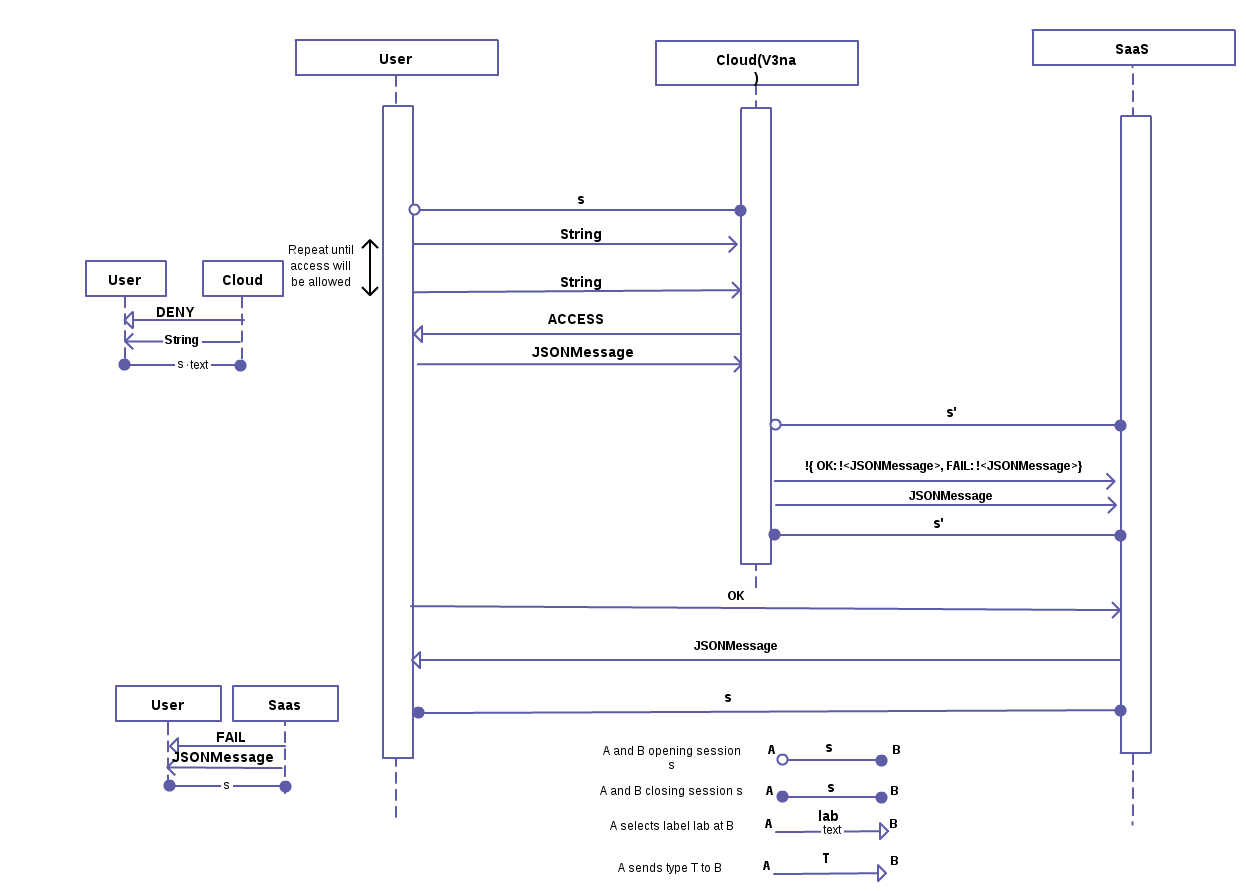
\includegraphics[width=0.8\textwidth]{interaction-sc2.png}
\caption{Sequence diagram of interactions for Scenario \# 2}
\label{fig:}
\end{figure}

\paragraph{Implementation.} Despite the fact that session delegation takes place, the program still remains very simple. Actually delegating the protocol is straightforward and only consists of passing the socket to service:

\begin{lstlisting}
s_vs.send(user_vu); // pass the remaining protocol
\end{lstlisting}

I have decided to include the whole segment of code to illustrate the following point. 

\begin{lstlisting}
user_vu.outbranch(ACCESS) {
  JSONMessage req_info = user_vu.receive();
  SJServerAddress addr_vs = SJServerAddress.create(p_vs, saas_hname, saas_port);
  SJSocket s_vs = SJRSocket.create(addr_vs); try(s_vs) {
    s_vs.request();
    s_vs.send(user_vu); // pass the remaining protocol    
    s_vs.send(req_info);
  } catch(UnknownHostException uhe) {
    uhe.printStackTrace(); 
  }
}
\end{lstlisting}

To receive a high order message type casting must take place in the case of a protocol, the type of protocol must be explicitly defined:

\begin{lstlisting}
v3na_user_socket = (@p_msg) v3na_sv.receive();
\end{lstlisting}

Where p\_msg is defined in the protocols section. This is a reason why it is good practice to first exclusively write the protocol to be delegated and then include it in the final protocol.

%------------------------------------------------------------------------------


\section{Intercloud Communication}
\label{sect:highlights}



%------------------------------------------------------------------------------
% Refs:
%
\label{sect:bib}
\bibliographystyle{plain}
%\bibliographystyle{alpha}
%\bibliographystyle{unsrt}
%\bibliographystyle{abbrv}
\bibliography{easychair}

%------------------------------------------------------------------------------
\appendix



%------------------------------------------------------------------------------
% Index
%\printindex

%------------------------------------------------------------------------------
\end{document}

% EOF
